% Glaubenskrieg — CTM Architecture Diagram for Paper
% Compile: pdflatex ctm_architecture.tex
% Output: ctm_architecture.pdf (to be included in paper)

\documentclass[tikz,border=3pt]{standalone}
\usepackage{amsmath,amssymb}

\definecolor{ctmblue}{HTML}{0062FF}
\definecolor{ctmorange}{HTML}{FF832B}
\definecolor{ctmgreen}{HTML}{24A148}
\definecolor{ctmred}{HTML}{FA4D56}
\definecolor{ctmpurple}{HTML}{8A3FFC}
\definecolor{ctmteal}{HTML}{009D9A}

\usetikzlibrary{arrows.meta,positioning,fit,backgrounds}

\begin{document}

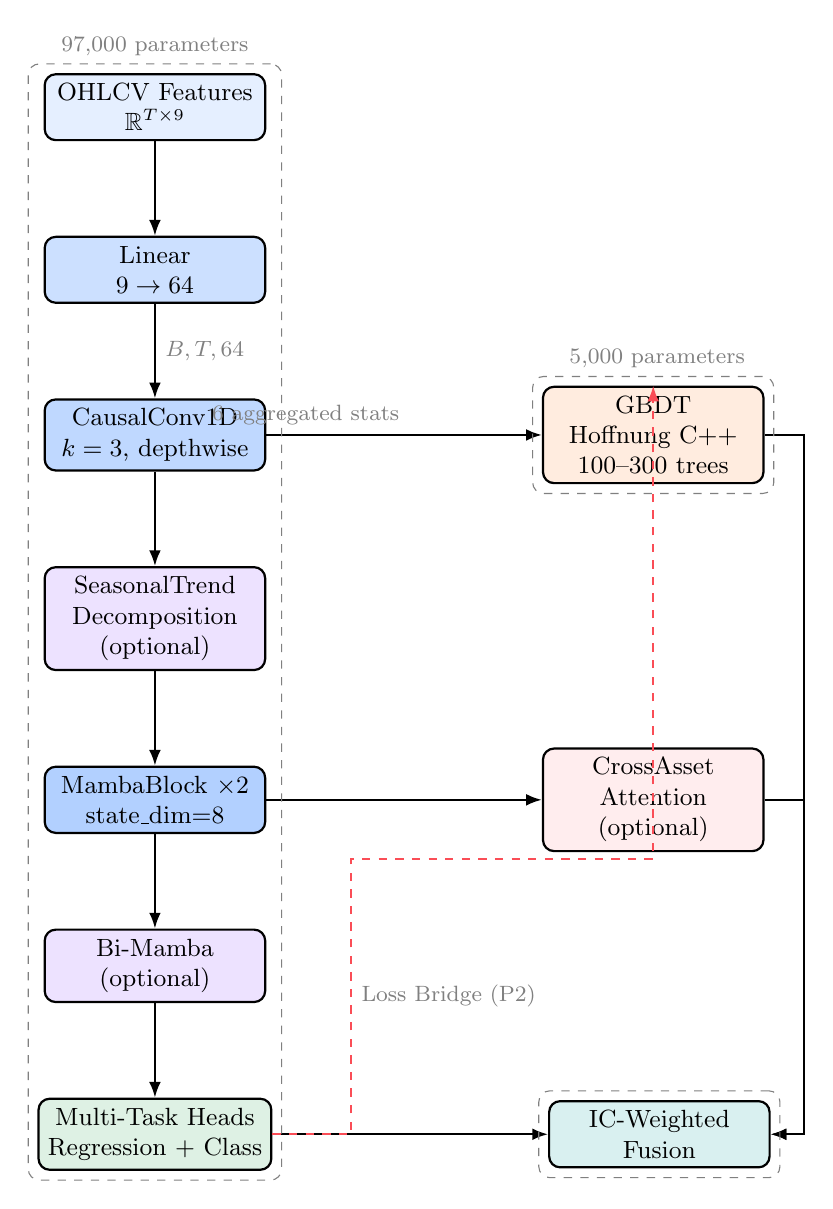
\begin{tikzpicture}[
    node distance=1.2cm and 1.5cm,
    block/.style={draw, rounded corners, thick, minimum width=2.8cm,
                  minimum height=0.8cm, align=center, font=\small},
    arrow/.style={-{Latex[length=2mm]}, thick},
    label/.style={font=\footnotesize, color=gray}
]

% ── Core CTM Path (left column) ──
\node[block, fill=ctmblue!10] (input) {OHLCV Features\\$\mathbb{R}^{T \times 9}$};

\node[block, fill=ctmblue!20, below=of input] (proj) {Linear\\$9 \to 64$};

\node[block, fill=ctmblue!25, below=of proj] (conv) {CausalConv1D\\$k=3$, depthwise};

\node[block, fill=ctmpurple!15, below=of conv] (decomp) {SeasonalTrend\\Decomposition\\(optional)};

\node[block, fill=ctmblue!30, below=of decomp] (mamba) {MambaBlock $\times 2$\\state\_dim=8};

\node[block, fill=ctmpurple!15, below=of mamba] (bi) {Bi-Mamba\\(optional)};

\node[block, fill=ctmgreen!15, below=of bi] (heads) {Multi-Task Heads\\Regression + Class};

% ── GBDT Path (right column) ──
\node[block, fill=ctmorange!15, right=3.5cm of conv] (gbdt) {GBDT\\Hoffnung C++\\100--300 trees};

\node[block, fill=ctmteal!15, right=3.5cm of heads] (fusion) {IC-Weighted\\Fusion};

% ── Cross-Asset Attention (between columns) ──
\node[block, fill=ctmred!10, right=3.5cm of mamba] (cross) {CrossAsset\\Attention\\(optional)};

% ── Arrows (CTM core) ──
\draw[arrow] (input) -- (proj);
\draw[arrow] (proj) -- node[label, right] {$B,T,64$} (conv);
\draw[arrow] (conv) -- (decomp);
\draw[arrow] (decomp) -- (mamba);
\draw[arrow] (mamba) -- (bi);
\draw[arrow] (bi) -- (heads);

% ── Arrows (GBDT path) ──
\draw[arrow] (conv.east) -- ++(0.5,0) |- (gbdt.west) node[label, midway, above] {6 aggregated stats};
\draw[arrow] (mamba.east) -- ++(0.5,0) |- (cross.west);

% ── Fusion arrows ──
\draw[arrow] (heads.east) -- ++(1.0,0) |- (fusion.west);
\draw[arrow] (gbdt.east) -- ++(0.5,0) |- (fusion.east);
\draw[arrow] (cross.east) -- ++(0.5,0) |- (fusion.east);

% ── Loss Bridge ──
\draw[arrow, dashed, ctmred] (heads.east) -- ++(1.0,0) 
    -- ++(0,3.5) node[label, midway, right] {Loss Bridge (P2)} 
    -| (gbdt.north);

% ── Annotations ──
\node[label, above=0.1cm of input] {97,000 parameters};
\node[label, above=0.1cm of gbdt] {~5,000 parameters};

% ── Section labels ──
\node[draw, dashed, rounded corners, fit={(input)(proj)(conv)(decomp)(mamba)(bi)(heads)},
      label={[ctmblue, font=\bfseries]above:CTM (Mamba SSM)}] {};
\node[draw, dashed, rounded corners, fit={(gbdt)},
      label={[ctmorange, font=\bfseries]above:GBDT}] {};
\node[draw, dashed, rounded corners, fit={(fusion)},
      label={[ctmteal, font=\bfseries]above:Ensemble}] {};

\end{tikzpicture}

\end{document}
